\chapter{\uppercase{Placa electrònica d'adquisició de dades i comunicació}}
Tal com s'indica als objectius del projecte part del treball consisteix en desenvolupar una placa electrònica encarregada d'adquirir dades, en aquest cas de freqüència cardíaca. \\
\newline Es vol que aquestes dades siguin accessibles i per això s'ha optat per dotar la placa d'un component de comunicació Wi-Fi gràcies al qual es podrà visualitzar una pàgina web amb les dades mesurades.\\
\newline La placa disposa d'una part d'alimentació que s'encarrega d'adaptar les tensions als nivells correctes dels diversos components. Existeix comunicació I2C entre els dos microcontroladors. Un s'encarrega d'adquirir les dades i tractar-les, mentre que l'altre està dedicat a la comunicació Wi-Fi.\\
\newline D'aquesta manera es poden realitzar tasques en paral·lel, cosa que seria impossible de fer amb un sol microcontrolador. Així, el microcontrolador que s'encarrega de la comunicació Wi-Fi pot esta donant servei a un client mentre el microcontrolador de l'Arduino Nano mostreja la senyal analògica.\\
\newline Si s'intentés fer tot amb un sol microcontrolador, podria ser que durant la dècima de segon que es necessita per donar servei al client ens perdéssim un batec. La fiabilitat del sistema disminuïra, i no ho volem.\\
\newline De forma esquemàtica es pot explicar el hardware mitjançant blocs.

\tikzstyle{decision} = [diamond, aspect=2, draw, fill=orange!20, 
    text width=4.5em, text badly centered, node distance=4cm, inner sep=0pt]
\tikzstyle{block} = [rectangle, draw, fill=red!40, 
    text width=5em, text centered, rounded corners, minimum height=5em]
    
\tikzstyle{block2} = [rectangle, draw, fill=green!40, 
    text width=7em, text centered, rounded corners, minimum height=3em, minimum width=7 em]
    
\tikzstyle{punt} = [rectangle, draw, fill=green!40, 
    text width=0em, text centered,  minimum height=0em, minimum width=0 em]
    
\tikzstyle{line} = [draw, -latex']
\tikzstyle{cloud} = [draw, ellipse,fill=red!20, node distance=3cm,
    minimum height=2em]
    
\begin{figure}[H]
\begin{center}
\begin{tikzpicture}[node distance = 2cm, auto, scale=0.65, every node/.style={scale=0.65}]
    % Place nodes
    \node [block] (pila) {Bateria (2,4 V)};  
    \node [block, right of=pila, node distance=5cm] (boost) {Convertidor Boost (5 V)};  
    \node [block, right of=boost, node distance=5cm] (buck) {Convertidor lineal (3,3 V)};  
    
    \node [block2, below of=boost, node distance=4cm] (nano) {Arduino Nano}; 
    \node [block2, left of=nano, node distance=6cm] (anell) {Anell de LEDs}; 
    \node [block2, below of=buck, node distance=4cm] (esp) {ESP-01}; 
    \node [block2, right of=esp, node distance=6cm] (ad8232) {AD8232};        

    % Draw edges
    \path [line] (pila) -- node [above] {2,4 V} (boost);
    \path [line] (boost) -- node [above] {5 V} (buck);
    
    \path [line] (boost) -- node [right] {5 V} (nano);
    \path [line] (boost) -- node [left] {5 V} (anell);
    \path [line] (buck) -- node [right] {3,3 V} (esp);
    \path [line] (buck) -- node [right] {3,3 V} (ad8232);
    
    \path [line] (nano) -- node [above] {DMX} (anell);
    \path [line] (nano) -- node [above] {bpm} (esp);
    

    \draw [->] (ad8232) to[bend left] node[auto] {Senyal analògica} (nano);
        
\end{tikzpicture}
\end{center}
\caption{Esquema de blocs del hardware}
\label{fig:organigrama}
\end{figure}

\section{Alimentació}
% Comentar com s'aliment placaa la. Afegir l'equip a amidaments i pressupost.
L'etapa de potència del nostre equip s'encarrega de transformar la tensió d'aproximadament 2,4 V de dues piles en sèrie a 5 V mitjançant un convertidor Boost que admet una tensió d'entrada mínima de 1 V i pot donar fins a 500 mA a la seva sortida de 5 V. Té una eficiència elevada i la seva sortida és constant. Les dimensions són acceptables.
\begin{figure}[H]
\begin{center}
\includegraphics[scale=0.25]{images/5V.jpg}
\end{center}
\caption{Regulador de tensió 5 V}
\label{fig: 5v}
\end{figure}
\noindent Algunes característiques del regulador són les indicades a la Taula \ref{tab:regulador}.
\begin{table}[H]
\small
\begin{center}
 \begin{tabular} {|l|r|}%{X | c c c} 
 \hline
 Característica & Valor \\
 \hline \hline 
Tensió de sortida & 5 V \\ \hline
Corrent màxim de sortida & 500 mA\\ \hline
Tensió mínima d'entrada & 1 V \\ \hline
Precisió de regulació de voltatge & 1\% \\ \hline
Tensió màxima d'entrada & 5 V \\ \hline
Topologia & Boost, font commutada \\ \hline
 \end{tabular}
 \caption{Característiques del regulador de tensió de la pila}
 \label{tab:regulador}
\end{center}
\end{table}
%\si\ohm
\noindent No n'hi ha prou de tenir 5 V a la sortida d'aquest convertidor. Els 5 V són necessaris per alimentar l'Arduino Nano, ja que el seu microcontrolador ATMEGA328 funciona a 5 V. La petita placa que conté l'ESP8266 i la placa de l'ADS8232 van alimentades a 3,3 V. Per tant, és necessari disposar d'una tensió d'alimentació de 3,3 V.\\
\newline El més directe seria fer servir el pin de 3,3 V de l'Arduino Nano, però comportaria un gran perill per aquesta placa de desenvolupament. Els 3,3 V de l'Arduino Nano venen d'un pin del mateix xip ATMEGA328. La màxima intensitat de sortida que pot donar és de 50 mA. El component ESP8266 consumeix, en funcionament normal, uns 70 mA, així que no és una solució.\\
\newline S'opta per un regulador lineal de bona eficiència anomenat AMS1117-3.3. Està especialment pensat per passar de tensions de 5 V a 3,3 V, que és exactament el que necessitem. A la seva entrada hi connectarem un condensador de 10 uF, així com a la seva sortida. Aquests condensadors evitaran la caiguda de tensió a la sortida en pics d'intensitat a la sortida.\\
\newline S'ha escollit aquest component amb el package SMD per tal d'optimitzar al màxim l'espai.
\begin{figure}[H]
\begin{center}
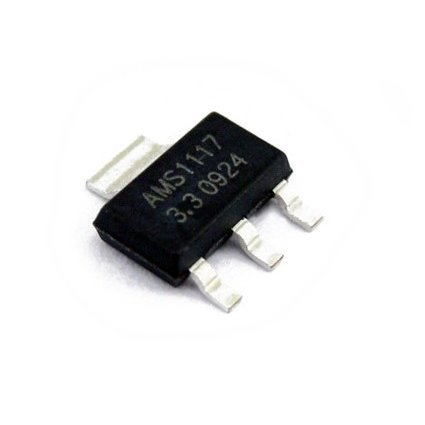
\includegraphics[scale=0.35]{images/ams3v3.jpg}
\end{center}
\caption{Regulador de tensió 3,3 V AMS1117 3,3}
\label{fig: 3v3}
\end{figure}
%
%
\noindent Algunes característiques del regulador són les indicades a la Taula \ref{tab:regulador2}.
\begin{table}[H]
\small
\begin{center}
 \begin{tabular} {|l|r|}%{X | c c c} 
 \hline
 Característica & Valor \\
 \hline \hline 
Tensió de sortida & 3,3 V \\ \hline
Corrent màxim de sortida & 800 mA\\ \hline
Tensió d'entrada & 5 V \\ \hline
Precisió de regulació de voltatge & 1,4\% \\ \hline
Topologia & Lineal \\ \hline
 \end{tabular}
 \caption{Característiques del regulador de tensió de 5 V a 3,3 V}
 \label{tab:regulador2}
\end{center}
\end{table}
%
\noindent Noteu els 800 mA màxims de sortida. Si considerem que la placa amb l'ESP8266 pot arribar a, com a màxim, pics de 200 mA i que la placa d'instrumentació té consums habituals de 170 uA (si no es considera el LED que pot tenir en alguns models comercials), no hi ha dubte que aparentment no hi ha problemes.\\
\newline En resum, podem mostrar una imatge que il·lustra de forma bastant intuïtiva les connexions d'aquests equips d'alimentació. Permeten adaptar la tensió de la pila als diferents nivells que requereixen les diferents plaques.
\begin{figure}[H]
\begin{center}
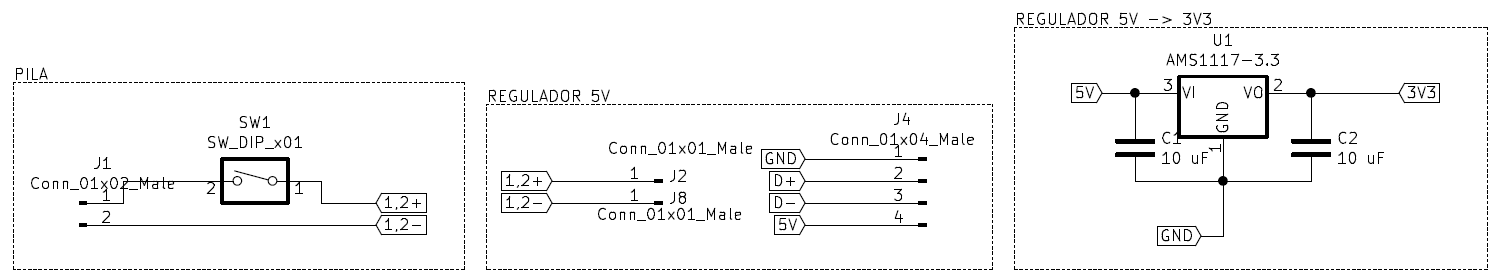
\includegraphics[scale=0.30]{images/alimentacio_2.png}
\end{center}
\caption{Etapes de potència de l'equip}
\label{fig:alimentacio}
\end{figure}

\section{Instrumentació}
% Insistir en la part d'instrumentació, posar equacions i indicar càlculs seguits
% Discutir per què s'ha escollit un OP AMP o un altre i així
La part d'instrumentació de la placa dona una senyal analògica a partir de la senyal captada als tres elèctrodes. Per això es fa servir una placa de desenvolupament que conté un integrat anomenat AD8232.

\begin{figure}[H]
\begin{center}
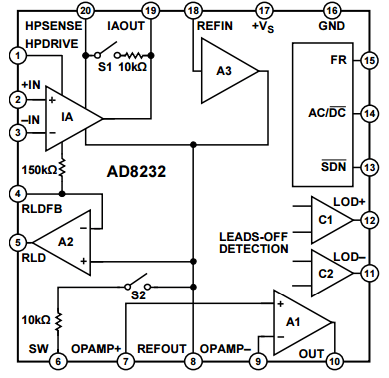
\includegraphics[scale=0.50]{images/ad8232_blocs.png}
\end{center}
\caption{Diagrama de blocs de l'integrat AD82332}
\label{fig:ad8232}
\end{figure}
%
%
\noindent En essència, el que es fa és alimentar la placa i llegir les tensions als tres elèctrodes. Dues d'aquestes tensions es resten i el resultat s'amplifica amb un amplificador diferencial, la referència del qual és el tercer elèctrode.

\begin{figure}[H]
\begin{center}
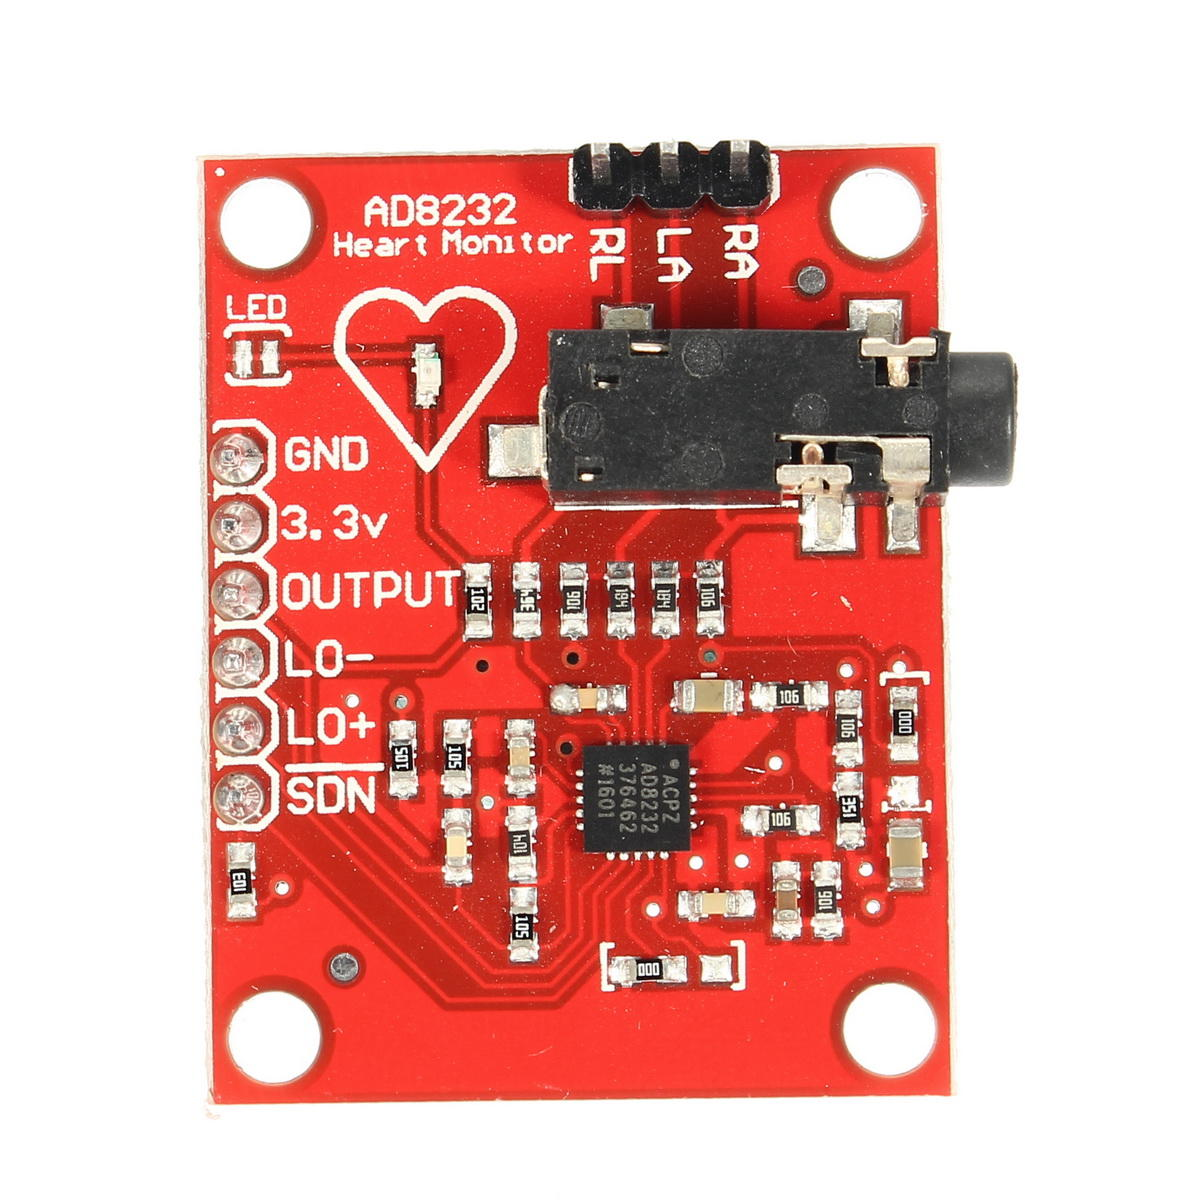
\includegraphics[scale=0.3]{images/ad8232.jpg}
\end{center}
\caption{AD8232 en una placa de desenvolupament}
\label{fig:ad8232}
\end{figure}
%
\noindent La sortida analògica de la placa que mostrem és fruit de les 3 tensions, tal com acabem d'explicar. Si les limitacions d'espai no fossin un problema es podria haver afegit un filtre pas baix per eliminar la freqüència de 50 Hz, provinent de la xarxa elèctrica.

\section{Anell de LEDs}
S'ha previst disposar d'un anell de LEDs per visualitzar de forma ràpida i intuïtiva la freqüència cardíaca de la persona que porti el dispositiu. Per bé que no podrà conèixer amb excessiva precisió la freqüència cardíaca de la persona, se'n pot fer una bona idea.\\
\newline L'anell que s'ha escollit és de la casa SparkFun. Té 16 LEDs 5050 disposats de forma circular. S'ha d'alimentar a 5 V i mitjançant un pin de DATA\_IN es pot fer el control dels colors de tots els LEDs així com de la seva intensitat llumínica i la seva saturació.\\
\newline Sparkfun té les seves llibreries com a codi obert, de forma que és molt fàcil testejar exemples i entendre de forma pràctica com funcionen.

\begin{figure}[H]
\begin{center}
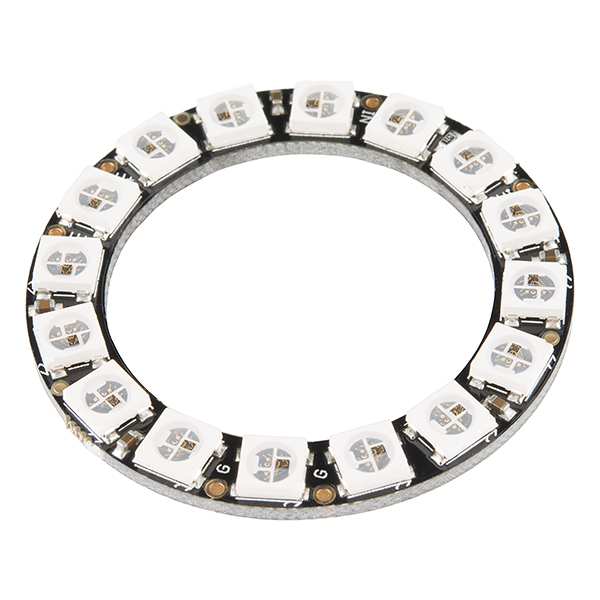
\includegraphics[scale=1.5]{images/led_ring.jpg}
\end{center}
\caption{Anell de LEDs}
\label{fig:ledring}
\end{figure}
%
\noindent La programació de l'anell s'ha fet de manera que cada LED té un color determinat. Si la freqüència és igual o més alta a la freqüència que simbolitza aquell LED, aquest s'encén. En cas contrari s'apaga. Cada vegada que hi ha un pols es fa com un refresc o "barrido" i s'encenen tants LEDs com cal. D'aquesta manera es dona una sensació de dinamisme.\\
\newline El consum d'aquest anell és de 18 mA segons indica el fabricant. Hem pogut comprovar que aquest número s'ajusta molt al mesurat a la realitat, i ens va sorprendre que fos així, ja que de normal un LED d'aquest tipus consumeix cap a uns 20 mA en funcionament normal.\\
\newline La raó que explica com és que el consum de 16 LEDs il·luminats a la vegada sigui tan baix és que cada LED s'il·lumina durant molt poc temps. Això es fa a alta freqüència i per tant l'ull humà ho interpreta com si cada LED sempre estigués encès.

\section{Comunicació}
% Explicar els diferents blocs lògics de la placa
L'ESP8266 permet establir comunicació Wi-Fi de forma efectiva. Després de fer algunes proves hem pogut determinar que el rang de comunicació possible de l'ESP8266 és proper al d'un telèfon mòbil convencional. La seva antena és una pista de circuit imprès. Actualment els mòbils també utilitzen aquest tipus d'antena.\\
\newline L'integrat ESP8266 muntat en una placa amb antena, cristall oscil·lador, resistències de pullup i condensadors de desacoblament es coneix com a ESP-01 i el seu pinout.
\begin{figure}[H]
\begin{center}
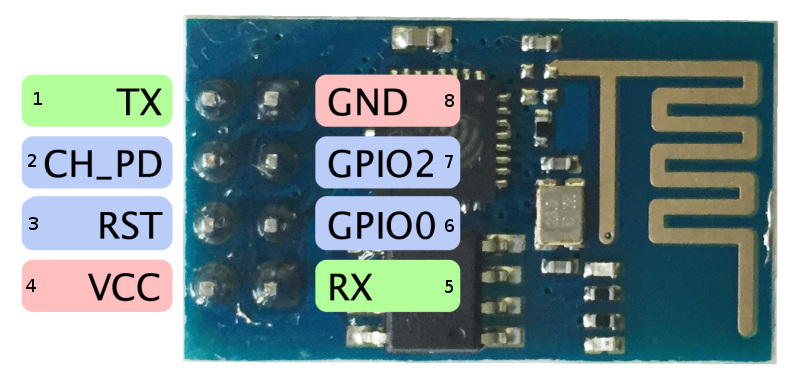
\includegraphics[scale=0.4]{images/esp01.jpg}
\end{center}
\caption{ESP-01}
\label{fig:ledring}
\end{figure}
%
\noindent El fet de què aquesta placa només tingui 8 pins no vol dir que el component només tingui 8 pins, de fet en té al voltant de 30. La placa que utilitzem té dos pins d'alimentació, un pin de TX i un de RX, dos pins de caràcter general, un pin per fer reset i un pin per habilitar l'integrat.\\
\newline El fabricant indica que es deixi una àrea lliure de coure sota l'antena per evitar interferències i problemes de comunicació.\\
\newline Algunes característiques de l'ESP8266 venen donades a la Taula \ref{tab:ESP8266}.
\begin{table}[H]
\small
\begin{center}
 \begin{tabular} {|l|r|}%{X | c c c} 
 \hline
 Característica & Valor \\
 \hline \hline 
Certificació & Wi-Fi Alliance \\ \hline
Freqüència de treball & 2,4 GHz \\ \hline
Potència de l'emissor & 17 dBm \\ \hline
Llindar de potència del receptor & -75 dBm \\ \hline
Rang de tensió d'alimentació & 2,5 V a 3,6 V \\ \hline
Corrent en funcionament normal & 80 mA \\ \hline

 \end{tabular}
 \caption{Característiques de l'integrat de comunicació ESP-8266}
 \label{tab:ESP8266}
\end{center}
\end{table}
% \si\ohm

\noindent D'aquí la importància d'alimentar-lo amb 3,3 V enlloc dels 5 V que ens arriben a la sortida del primer regulador. Per això es fa servir el regulador de tensió que passa de 5 V a 3,3 V.\\
\newline Un altre aspecte a destacar és la tensió dels pins digitals. En el nostre cas s'estableix comunicació I2C entre l'ESP-01 i l'Arduino Nano. Els pins digitals de l'Arduino Nano treballen a 5 V i els de l'ESP-01 en principi estan pensats per treballar a 3,3 V, que és la seva tensió d'alimentació. Així, podria haver-hi problemes si no es fes servir un adaptador de tensions. El fabricant de l'ESP-01, però, ja va preveure que podria haver-hi conflicte i assegura que els pins digitals poden estar a 5 V sense problema de danyar l'integrat.

\section{Circuit imprès}
% Questions de PCB, clearance i tal
S'ha dissenyat un PCB a doble cara que conté les parts electròniques que s'han anat comentant.\\
\newline Per bé que es podria haver ajuntat els esquemàtics de totes les plaques d'avaluació que fem servir en una sola placa de circuit imprès, això hauria portat un temps considerable per adquirir tots els components i testejar-los. A més, alguns components ens hauria sigut molt difícil, per no dir impossible, de soldar manualment.\\
\newline Si aquest projecte seguís endavant i tingués el finançament necessari, llavors sens dubte s'optaria per contractar un servei integral en què ens fessin el PCB i ens hi soldessin els components.\\
%
%
%
\newline Les pistes d'alimentació s'han fet més gruixudes que les de senyal digital. Les pistes de tensió de les plaques s'han fet una mica més gruixudes, tot i que la intensitat a través seu és petita. La separació d'una d'aquestes pistes amb la resta és generosa per evitar l'arc elèctric. A més, es preveu recobrir la placa amb una pel·lícula, cosa que disminuiria encara més el risc d'arc elèctric.\\
\newline La majoria de components són SMD. Solen ser més barats i ocupen molt menys espai en comparació als components que travessen la placa. Així, les dimensions finals de la placa són de 4,5 x 4,1 cm aproximadament.\\
\newline S'han seguit especificacions del fabricant pel disseny de la part de RF. Pel disseny de la part d'instrumentació s'ha tingut especial cura en utilitzar condensadors de desacoblament a les alimentacions dels integrats i situar-los prop d'aquests.\\
\newline La vista superior de com quedaria la placa és la de la Figura \ref{fig:3d_sup}.
\begin{figure}[H]
\begin{center}
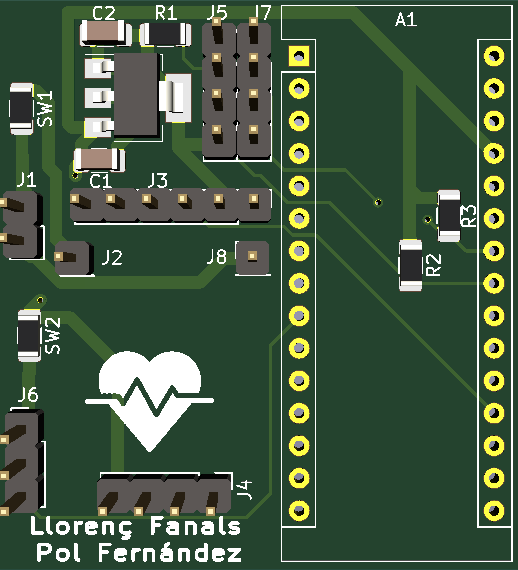
\includegraphics[scale=0.4]{images/placa.png}
\end{center}
\caption{Vista 3D de la cara superior de la placa}
\label{fig:3d_sup}
\end{figure}

\noindent No es disposa del model 3D de l'Arduino Nano.\\
\newline Es pot observar com figuren una gran quantitat de connectors. La majoria simbolitzen allà on aniran connectades les plaques de desenvolupament. Algunes aniran amb pins de gran longitud per aconseguir tenir, a part d'aquesta placa "base", dos nivells més de plaques.\\
\newline D'aquesta manera s'intenta optimitzar l'espai el màxim possible. Si es col·loquessin totes les plaques de desenvolupament de costat el resultat seria un equip amb molt poc gruix però molta superfície.\\
\newline La serigrafia de què s'ha dotat la placa facilita les connexions de les diferents plaques de desenvolupament.\\
\newline Pel que fa a la cara inferior, aquesta es mostra a la Figura \ref{fig:inf}. Aquesta cara s'utilitza per fer passar alguna pista que d'altra manera congestionaria la cara superior. Per passar d'una capa a l'altra es fan servir via's. La resta de la cara superior conté el pla de massa i forats pels components through-hole.

\begin{figure}[H]
\begin{center}
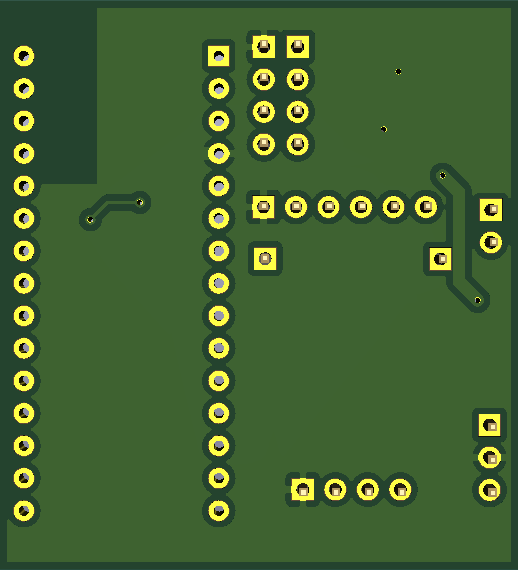
\includegraphics[scale=0.4]{images/placa2.png}
\end{center}
\caption{Vista de la cara inferior de la placa}
\label{fig:inf}
\end{figure}
\noindent Hem decidit encarregar aquesta placa a Xina. Per uns 20 € hem aconseguit 5 unitats i amb transport ràpid. El fabricant, JLCPCB, ha fabricat la placa en menys de 24 hores. L'enviament ha durat uns 3 dies. Considerem el resultat molt satisfactori:
\begin{figure}[H]
\begin{center}
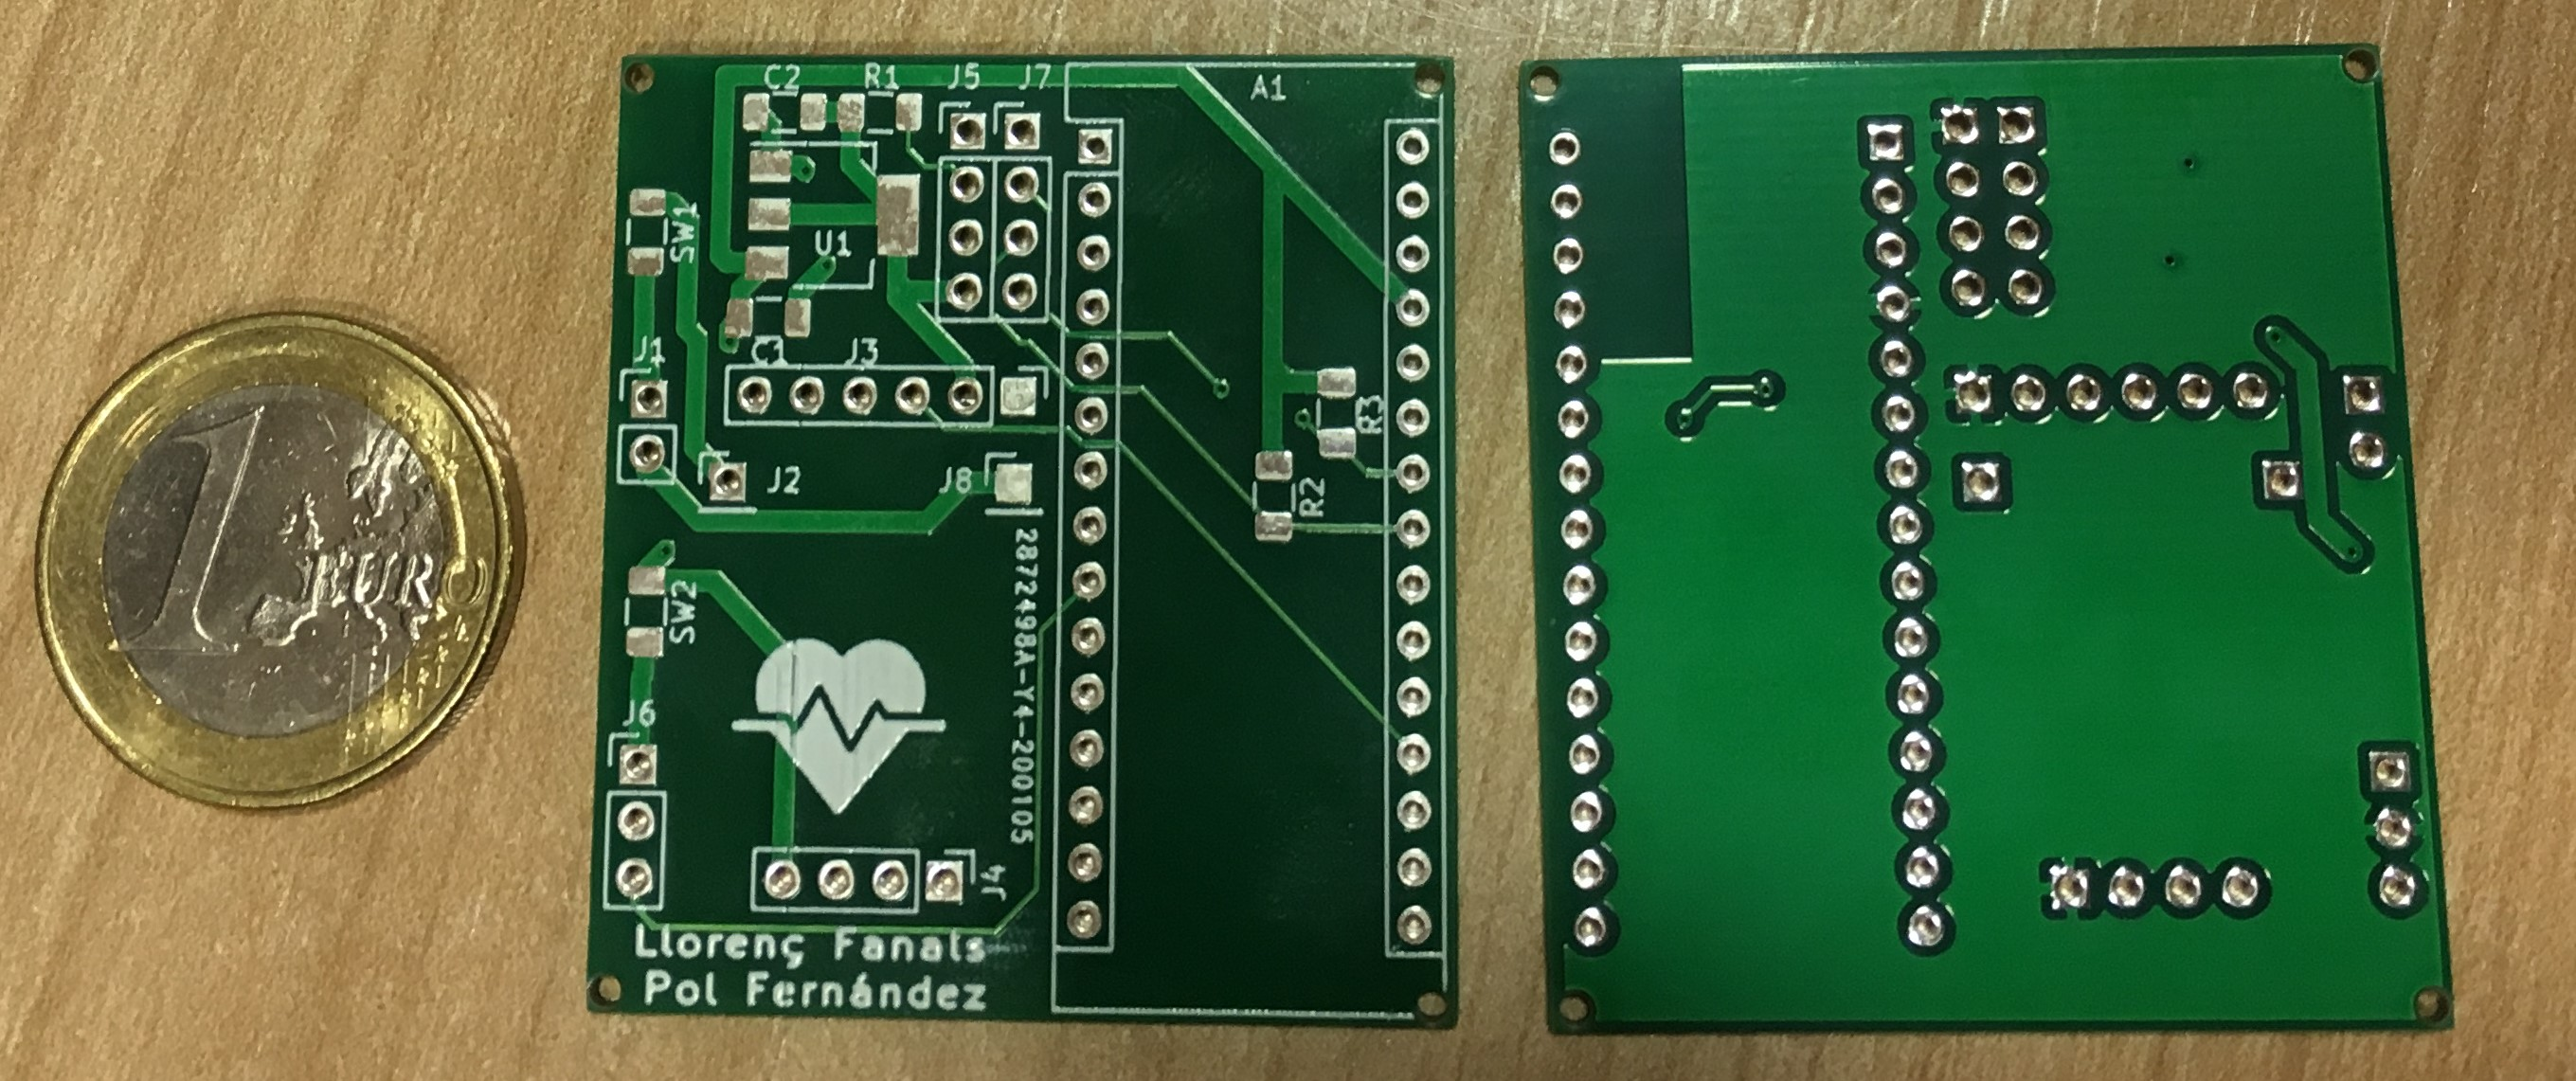
\includegraphics[scale=0.15]{images/pcb_fisic.jpg}
\end{center}
\caption{Vista de les dues cares del PCB}
\label{fig:inf}
\end{figure}

\clearpage


% Table generated by Excel2LaTeX from sheet 'Hoja1'
%\begin{table}[H]
%  \centering
%    \begin{tabularx} {\textwidth} {|X|r|} \hline
%  \multicolumn{1}{|c|}{Descripció} &  \multicolumn{1}{c|}{Quantitat}\\ \hline \hline
%
 %   Placa GLC 330 W & 10 \\ \hline
%    Inversor FRONIUS Primo 3.0-1 Light 3kW & 1 \\ \hline
%    Metres cable Ethernet RJ-45 CAT 8 & 10 \\ \hline
%    Metres cable 4 m$m^2$ PVC & 45 \\ \hline
 %   Metres cable 1,5 m$m^2$ PVC & 100 \\ \hline
 %   Punteres Enghofer E 4-10, 4 m$m^2$, 10 mm & 20 \\ \hline
 %   Punteres Enghofer E 1.5-10 1,5 m$m^2$ 10 mm & 12 \\ \hline
 %   Cinta aïllant 10 m 1,6 cm & 3 \\ \hline
 %   Caixa estanca Solera CONS 100x100x55 mm & 2 \\ \hline
  %  Canal Euroquint 25,16 mm 1,5 metres & 20 \\ \hline
%    Curva canal VECAMCO & 10 \\ \hline
%    Paquet de 50 brides 200x2,6  mm & 2 \\ \hline
%    Regleta nylon 12 pols 16 mm & 4 \\ \hline
%    Premsaestopes M12 & 10 \\ \hline
%    Cargol autoroscant M4 16 mm & 12 \\ \hline
%    Tacs Fischer 072095 nylon 6x50 mm & 50 \\ \hline
%    Díode SM74611KTTR & 10 \\ \hline
%            Hores enginyer & 1 \\ \hline
%    Hores oficial de primera & 12 \\ \hline
%    Hores oficial de segona & 12 \\ \hline
%    \end{tabularx}%
%  \label{tab:addlabel}%
% \end{table}%
